
\chapter{Project Results }
\section{Physical objective}
The aim is to construct a loudspeaker system with a flat response due to the accuracy and quality of the filters, the amplifier, and the power supply.\\
We should be able to plug the speaker in and have music come out of it. The music should be split between 3 speakers: high frequencies come out of the tweeter, middle frequencies come out of the mid-speaker, and low frequencies from the woofer.\\
We should also be able to have an additional active filter for the bass level. 


\begin{itemize}
    \item Power supply: The power supply sub-group needs to create a circuit that brings down the input voltage of 230 volts to an average of 19 volts. Afterward, the AC input has to be transformed into a stable DC output. 
    \item Power amplifier: The power amplifier group have to filter out the bandwidth for the high/mid/low pass filters. Therefore the values of the capacitors and resistors must be chosen carefully to get the right bandwidth
    \item High/mid/low pass filters; The high/mid/low pass filters sub-groups need to filter out their specific frequencies. The filtered frequencies of the high, mid, and low pass filters should line up perfectly next to each other in order to prevent gaps or overlapping. 
\end{itemize}

    
    


\section{Learning objectives}
Besides creating a working sound system, the goal is to master certain learning objectives of the EPO project. After completion of the project, we will be able to apply the theoretical concepts of the first semester in practice.\\
Next, we have to achieve the basics of working in an engineering project group. the basics consist of planning, creating well-organized meetings, writing project plans, having the ability to give presentations, and writing engineering reports.\\
At last, we will achieve academic skills on a level that is expected of the university. for example being able to address specific problems, analyze data sheets and manuals, and critically assess and cit ate information.

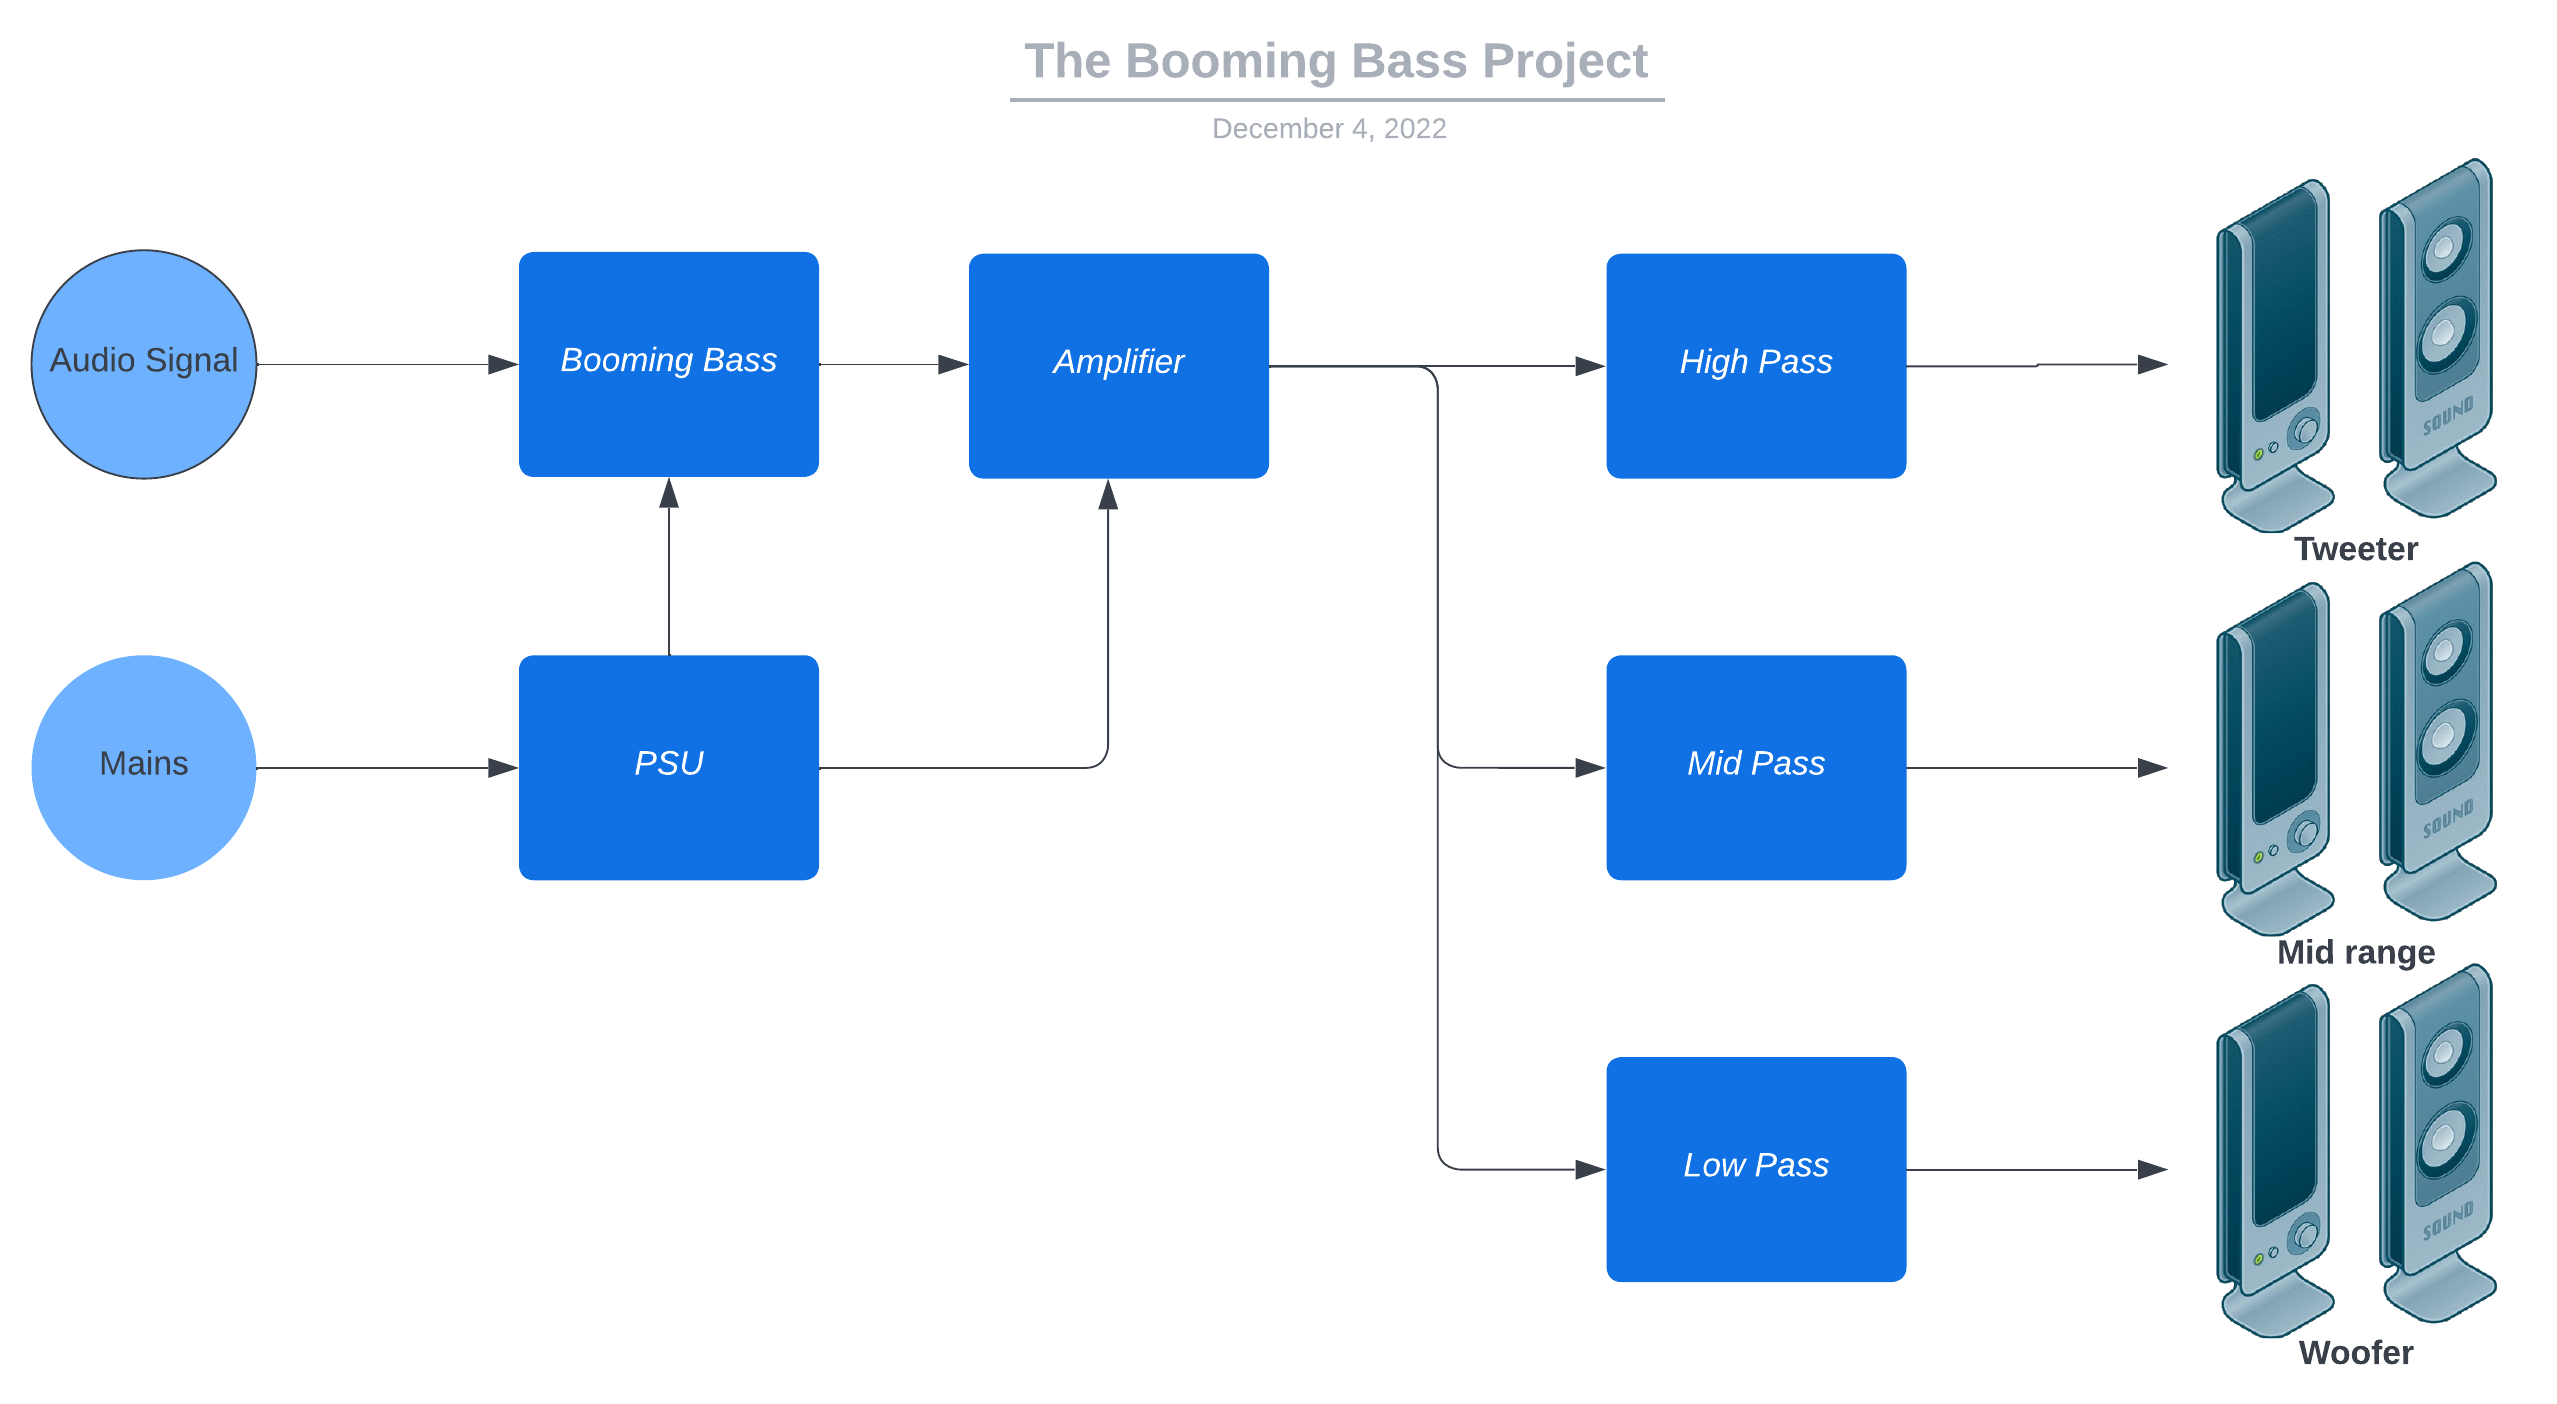
\includegraphics[scale=0.72]{Flowchart_1.png}









